\documentclass[11pt]{report}

\usepackage{graphicx}
\usepackage[utf8x]{inputenc}
\usepackage{grffile}
\usepackage[margin=1in]{geometry}
\usepackage{multicol}
\usepackage{afterpage}
\usepackage[english]{babel}
\usepackage{caption}
\usepackage{subcaption}
\usepackage{pgfplots}
\usepackage{pgf-pie}
\usepackage{hyperref}
\usetikzlibrary{shadows}

\setlength{\parindent}{0pt}

\begin{document}

\afterpage{
\newgeometry{}
\begin{titlepage}
\centering

\mbox{
\textsc{\LARGE Universit\`a degli Studi del Piemonte Orientale}
}\\[.2cm]
\textsc{\LARGE ``Amedeo Avogadro''}
\begin{figure}[htp]
\centering
\includegraphics[scale=2]{img/logo_uniupo.png}
\label{}
\end{figure}

\mbox{
\textsc{\Large Dipartimento di Scienze ed Innovazione Tecnologica}
}\\[1cm]

\Large Corso di Laurea in Scienze Biologiche\\
\textsc{\Large Prova Finale}\\[1.5cm]

{\LARGE \bfseries Genotypic Evaluation of \\Carbapenemases Producing Strains \\[0.2cm]Isolated from Different Biological Materials}

\vfill

% Authors
\begin{multicols}{2}
\begin{flushleft}
	{\Large Relatrice:\\
	Prof.ssa Elisa Gamalero\\[0.5cm]
	Tutor Aziendale:\\
	Dott. Andrea Rocchetti}
\end{flushleft}
\columnbreak
\begin{flushright}
	{\Large Candidata:\\
	Simona Debilio}
\end{flushright}
\end{multicols}
\vspace{1cm}
Anno Accademico 2016 -- 2017
\vspace{-2cm}

\end{titlepage}
\clearpage
\restoregeometry
}

\tableofcontents

\chapter{Introduction}
One of the most important discoveries in human history has been the identification of substances that were able to fight and defeat bacterial infections.
These substances, called ``antibiotics'', had an extraordinary impact on the outcome of bacterial infections and, consequently, helped to extend life expectancy \cite{ventola2015antibiotic}.

The first antibiotic was penicillin, discovered by Sir Alexander Fleming in 1928 (Figure \ref{fleming}) and following developed by chemical companies.

%autore foto non trovato
\begin{figure}[htp]
\centering
\includegraphics[scale=1.10]{img/fleming.jpg}
\caption{``It has been demonstrated that a species of penicillium produces in culture a very powerful antibacterial substance which affects different bacteria in different degrees.
Generally speaking it may be said that the least sensitive bacteria are the Gram-negative bacilli, and the most susceptible are the pyogenic cocci. [...]
In addition to its possible use in the treatment of bacterial infections penicillin is certainly useful [...] for its power of inhibiting unwanted microbes on bacterial cultures so that penicillin insensitive bacteria can readily be isolated.''\\
Alexander Fleming}
\label{fleming}
\end{figure}

\clearpage
At first, antibiotics were used to treat serious infections in the 1940s, and they had similar positive outcomes worldwide \cite{Spellberg2014}.

Unfortunately, after many decades since the use of the first antibiotics on patients, bacterial infections began to spread again and, more importantly, became a threat again.
This renewed spread of bacterial infections is due to the emergence of bacterial strains that are resistant to most of present antibiotics \cite{ventola2015antibiotic}.

The main causes that have provoked this antibiotic resistance crisis, which is occurring worldwide, are antibiotic overuse and misuse.
In addition, there has been a lack in the development of new drugs by the pharmaceutical industry \cite{nature2013}.
Overall, this situation has a huge impact on human health (Figure
\ref{spread2050}).

\begin{figure}[htp]
\centering
\includegraphics[scale=0.80]{img/spread2050.png}
\caption{In 2014 the UK Government commissioned the Review on Antimicrobial Resistance (AMR) to analyse the global problem of rising drug resistance.
The process was completed in two years and some projections, based on the data gathered, showed that an increase in infection rates could mean 150 million people dying between now and 2050 (Source: ``Antimicrobial Resistance: Tackling a Crisis for the Health and Wealth of Nations: December 2014'' \cite{review2014antimicrobial})}
\label{spread2050}
\end{figure}

As epidemiological studies have shown there is a direct relationship between the use of antibiotics and the emergence and spread of resistant bacteria strains \cite{huttner2013antimicrobial}.

Resistance can arise spontaneously through mutation (Figure \ref{mutation}), but it can also be acquired from genetic elements inherited from other bacteria.
The acquisition of mobile genetic elements (i.e. plasmids) is called ``horizontal gene transfer'', and it allows not only the transfer among different members of the same species, but also among members of different species.

Furthermore, antibiotics cause the death of drug sensitive competitors, leaving only the resistant bacteria alive and able to reproduce themselves as the result of natural selection \cite{doi:10.1093/emph/eou024}.

\clearpage
\begin{figure}[htp]
\centering
\includegraphics[scale=0.57]{img/mutation.png}
\caption{Most microbes can evolve rapidly thanks to their short reproductive cycle.
During these frequent replications, mutations can arise; some of them can help the microbe surviving the exposure to antibiotics (Source: ``Mutation Causes Drug Resistance'' \cite{mutation}).}
\label{mutation}
\end{figure}

One way we can limit the spread of antibiotic resistant strains is by minimising the natural selection for resistance genes.
This can be achieved by reducing the use of antibiotics, avoiding their use unless it is strictly necessary, and enhancing infection prevention (e.g. isolating infected patients, and improving the hygiene).

Moreover, it is necessary to stop abusing antibiotics in agriculture \cite{Spellberg2014} \cite{doi:10.1093/emph/eou024} (Figure \ref{farm}).
The excessive use of antibiotics in agriculture can lead to antibiotic resistance, due to the spread of molecules from the animal faeces to soil, water, and food.
This phenomenon can cause the involuntary ingestion of antibiotics in humans, and strengthening the natural selection for the microorganisms.

\begin{figure}[htp]
\centering
\includegraphics[scale=0.57]{img/farm.jpg}
\caption{Antibiotics, when given to animals, kill most of the bacteria living in their intestines.
Resistant strains can multiply and spread in the environment from their faeces \cite{farm}.}
\label{farm}
\end{figure}

\clearpage
Following the EU conference titled ``The Microbial Threat'', which took place in 1998 in Copenhagen, antibiotic resistance became an official EU issue for the first time.
Since 2001, the European Council has highlighted the importance of reinforcing epidemiological surveillance, and improved the supervision of laboratories.
The council also highlighted the need to create a coordinated structure at national level, in order to prevent and control the spread of antibiotic resistances.
In recent years Italy has seen the spread of Gram-negative bacteria, mostly belong to the \emph{Klebsiella pneumoniae} species that ascribed to the \emph{Enterobacteriaceae} family, have become resistant to carbapenems (e.g. Imipenem and Meropenem).

A dramatically increasing trend in resistance has been observed between 2009 and 2011: while only the 1,3$\%$ of \emph{K. pneumoniae} strains isolated from blood showed a resistance in 2009, the percentage rose to 16$\%$ in 2010, and 26.7$\%$ in 2011 respectively (Figure 1.5 e 1.6).

\begin{figure}[htp]
\centering
\includegraphics[scale=0.60]{img/K.pneu_2009.png}
\caption{Klebsiella pneumoniae: proportion of invasive isolates resistant to carbapenems in 2009 \cite{ECDC_Surveillance}.}
\label{}
\end{figure}

\clearpage
\begin{figure}[htp]
\centering
\includegraphics[scale=0.60]{img/K.pneu_2015.png}
\caption{Klebsiella pneumoniae: proportion of invasive isolates resistant to carbapenems in 2015 \cite{ECDC_Surveillance}.}
\label{}
\end{figure}

These studies have confirmed the recent spread of multiresistant Enterobacteria in Italy, and they have shown why these bacteria represent a concrete threat for public health, as they are frequently the cause of infections, both in hospital and community environment \cite{circolare2013}.

Clinical microbiology laboratories play an essential role in monitoring the spread of carbapenemase-producing Enterobacteria (CPE).
This role entails significant demands upon laboratory staff and resources.
For example, medical personnel must become familiar with a series of technical procedures for rapid identification of resistant bacterial strains in order to apply appropriate measures to contain their spread; this is required to allow effective and rapid application of appropriate infection controls in response.
The potential clinical impacts upon patients also requires microbiologists undergo constant methodological, technical and organizational training.
A timely identification of the antibiotic-resistant strains allows an effective implementation of control over a particular infection.

\section{The definition of infectious diseases and transmission}
Infectious diseases are caused by pathogens, such as bacteria, viruses and fungi.
When coming into contact with a host, pathogens are able to procreate and cause functional impairments.
Hence, diseases arise from these complex interactions between the host immune systems and the foreign organisms.
Parasitism is the relationship between pathogens and hosts, where the pathogens take advantage of some vital functions of the host to replicate and survive.

The human body is equipped with various defences against foreign substances and microorganisms.
For example, skin and mucous are first line defence that possess antimicrobial properties which allow them to serve as effective barriers against bacterial invasion.

The process of invasion and proliferation of infectious microorganisms within the host body is called infection.
Typically, there is an incubation period prior to the onset of a disease.
Incubation period is defined as the time elapsing from the exposure of an infectious agent and the first appearance of symptoms.
An incubation period can varies depending on the disease, and the establishment of the ``infectious agent-host'' relationships.

Infections may be symptomatic or asymptomatic.
A disease can be classified when symptoms appear during the infection; asymptomatic infections are also referred to as sub-clinical infections, where infected individuals can carry the disease without visible symptoms.

Contagious infectious diseases are caused by pathogens that are transmitted to receptive subjects.
Infectious diseases which are not contagious require instead the intervention of suitable vectors under specific circumstances.
Infectious diseases can be effectively prevented through either preventing exposure, or reducing susceptibility, to pathogens \cite{EPICentro}.

\chapter{What are antibiotics and how they work}
Antibiotics are secondary metabolites produced naturally by bacteria and other soil microorganisms.
They are thought to primarily play a defensive function in natural environments.
From a pharmacological point of view, antibiotics have revolutionised medicine, providing a universal cure for infectious diseases that were untreatable for centuries.
Hundreds of molecules with antibacterial activity have been identified over the last century.
They are divided into different classes based on different chemical characteristics that distinguish the pharmacologically active molecule.
Although every antibiotic interferes with the survival of the bacteria at various levels, their mechanisms of action may differ significantly from one species to another.
Antibiotics can alter the structures of bacterial cell wall or membrane, with the energy metabolism such as nucleic acids, and protein synthesis (Figure \ref{ant_targ}).

Depending on the types of antibiotic, there can be either bactericidal effects, that directly cause the death of microorganisms, or bacteriostatic effects, that cause the inhibition of the bacterial reproduction, but not their death \cite{Leekha2011}.

Antibiotics distinguish themselves from other substances of microbial origin (e.g. toxins) because they can present high selectivity with regard to bacterial cells and low toxicity to eukaryotic cells.
This mechanism is called selective toxicity.
It allows antibiotics to eliminate the infections without damaging the hosts.

Each antibiotic has its own spectrum of activities.
For example, some antibiotics are effective on Gram-positive bacteria, while others are effective on Gram-negative bacteria.
There are also broad-spectrum antibiotics, which could target many of the Gram-positive as well as Gram-negative bacteria.
There is, however, not a single antibiotic that is effective against all bacteria.
Consequently, knowledge of an antibiotic’s activity spectrum is required to define an effective and targeted pharmacological therapy.

\clearpage
\begin{figure}[htp]
\centering
\includegraphics[scale=0.4500]{img/ant_targ.png}
\caption{Antibiotics can have different modes of action: they can inhibit DNA, proteins, or cell wall synthesis, but they can also interfere with the bacterial metabolism, or cause the impairment of nucleic acids.
(Source: ``Microbiology: a clinical approach'' \cite{microbiology})}
\label{ant_targ}
\end{figure}

\section{$\beta$-lactam antibiotics}
$\beta$-lactam antibiotics are a class of broad-spectrum antibiotics that contain a $\beta$-lactam ring in their molecular structures.
The examples of $\beta$-lactam antibiotics are penicillin derivatives, cephalosporins and carbapenems \cite{Pitout2005}.
These antibiotics present a nucleus (6-aminopenicillanic acid) connected to different lateral chains that affect their pharmacokinetic peculiarities and their range of action (Figure \ref{beta_lact}).

Penicillins have a bicyclic structure, where the $\beta$-lactam ring is the functional part of the molecule: if degraded the drug loses its effectiveness.
$\beta$-lactam antibiotics are target many Gram-negative and Gram-positive bacteria by inhibiting bacterial cell wall biosynthesis.

Without cell wall, the bacterial cells would rupture due to the difference in osmolarity between the inside and the outside of the cell.

\clearpage
\begin{figure}[ht]
\label{beta_lactam} 
  \noindent\begin{minipage}[b]{0.5\linewidth}
    \includegraphics[width=.5\linewidth]{img/carbapenem.png} 
    \caption*{Carbapenems} 
  \end{minipage}%
  \noindent\begin{minipage}[b]{0.5\linewidth}
    \includegraphics[width=.5\linewidth]{img/cephalosporin.png} 
    \caption*{Cephalosporins} 
  \end{minipage}
  \noindent\begin{minipage}[b]{0.5\linewidth}
    \includegraphics[width=.5\linewidth]{img/penicillin.png} 
    \caption*{Penicillins}
  \end{minipage}%
  \hfill
  \noindent\begin{minipage}[b]{0.5\linewidth}
    \includegraphics[width=.5\linewidth]{img/aztreonam.png} 
    \caption*{Aztreonam} 
  \end{minipage}%
  \caption{$\beta$-lactam antibiotics are named after their $\beta$-lactam ring: this is a four membered lactam with a nitrogen atom attached to the $\beta$-carbon atom relative to the carbonyl.}
 \label{beta_lact}
\end{figure}


The substance that confers the resistance and rigidity to the cell wall is called peptidoglycan, an amino-sugar polymer.
Peptidoglycan forms a mesh-like layer, consisting of glycosaminoglycan chains that interlinked with short peptides.
The sugar component consists of alternating disaccharide of N-acetylglucosamine (NAG) and N-acetylmuramic acid (NAM), connected by a $\beta$(1,4) glycosidic linkage where the NAM is also attached to a chain of four amino acids (both D- and L-).

The repetitive polymer structure is resilient due to the third amino acid bonded to the NAM of a NAM-NAG chain, that is also tied to the fourth amino acid of a NAM on a parallel chain.
Penicillins block the formation of the cross-linking bonds within the peptidoglycan, therefore compromising their development in bacterial cell wall synthesis (Figure \ref{pept}).
The development of these bonds is catalysed by a class of enzymes called ``penicillin binding proteins'' (PBP).
These enzymes are able to remove one of the two residues of D-alanine placed at the end of the NAM pentapeptide.

$\beta$-lactam antibiotics are able to inhibit PBP enzymes via a competitive mechanism: the similarity of $\beta$-lactam antibiotics chemical structures to the D-alanine D-alanine dimer in peptidoglycan has allowed the antibiotics to become competitor substrates for PBP binding.
When the enzyme binds to the antibiotic, an acyl-enzyme stable complex will be formed; this inactivates the enzymatic activity where the PBP will no longer be capable of catalysing the peptidoglycan synthesis reactions, and lead to the death of the growing bacterial cells \cite{kong2010beta}.

\clearpage
\begin{figure}[htp]
\centering
\includegraphics[scale=0.50]{img/Peptidoglycan.jpg}
\caption{The peptidoglycan is synthesised in three different locations during three different stages: the first occurs in the cytoplasm, where the Lipid I is synthesised; the second takes place in the cytoplasmatic membrane where the Lipid I is transformed in the Lipid II and then flipped to the external side of the membrane, where the third stage occurs.
During the last stage the Lipid II is linked to the nascent peptidoglycan by PBPs \cite{Pinho2013}}
\label{pept}
\end{figure}

\subsection{Carbapenem antibiotics}
A new era of $\beta$-lactam antibiotics, the carbapenems, has begun after the discovery of \emph{Streptomyces cattleya} and its antibiotic product, thienamycin.
After thienamycin, numerous carbapenems were discovered (i.e. imipenem, meropenem) \cite{Birnbaum1985}.
Carbapenems belong to the class of $\beta$-lactam of antibiotics.
Unlike penicillins, carbapenems have a broader spectrum of activity, with greater effectiveness that is less likely to be affected by many of the most common mechanisms of antibiotic resistance.

This group of antibiotics presents a remarkable activity against both Gram-positive, and Gram-negative bacteria that include \emph{Enterobacteriaceae}, \emph{Pseudomonas aeruginosa}, and \emph{Bacteroides} \cite{Neu1985}.

Since carbapenems are more effective against infections caused by multidrug-resistant bacteria than other $\beta$-lactam antibiotics, they are primarily used in hospitalised patients.

\chapter{The antibiotic resistance and the $\beta$-lactamases}

The discovery and development of antibiotics are considered one of the major breakthroughs of modern medicine.
The role of antibiotics has been essential in treating bacterial infections, and saving many lives.
Unfortunately, time has seen the emergence and spread of antibiotic resistances among bacteria, weakening their effects.
The development of combined resistances to multiple classes of antibiotics have brought to strains with multidrug-resistance (MDR) phenotypes, which can render traditional antibiotics completely ineffective \cite{Rossolini2014}.

Since $\beta$-lactams were the first antibiotics to be discovered, the resistance to this type of antibiotics was the first to emerge, and to be understood.
The most effective way for bacteria to react to these antibiotics is by producing $\beta$-lactamases.
These enzymes are able to hydrolyse the $\beta$-lactam ring of the antibiotics and, consequently, to inactivate them \cite{kong2010beta}.

$\beta$-lactamases were traditionally classified based on either functional or structural characteristics in early studies.
More recently, these enzymes have been classified based upon their amino acid homology.
Four different molecular classes have been described; classes A, B, C and D.
Molecular classes A, C, and D include the $\beta$-lactamases with serine at their active site, whilst class B $\beta$-lactamases are all metallo-enzymes with an active-site zinc \cite{Queenan2007}.

\section{The carbapenemases}
Carbapenemases are part of the classes A, B, and D of $\beta$-lactamases.
They are highly adaptive in hydrolytic capacities compared to other members of $\beta$-lactamases.

\subsection{Class A carbapenemases}
Bacteria expressing class A serine carbapenemases have low susceptibility to imipenem, with a Minimum Inhibitory Concentration (MIC) that can range from mildly elevated to fully resistant.
There are three major families within the class A serine carbapenemases:

\begin{itemize}
\item not metalloenzyme carbapenemase (NMC);
\item imipenem-hydrolysing $\beta$-lactamase (IMI)/Serratia marcescens enzyme (SME); 
\item Klebsiella pneumoniae carbapenemase (KPC).
\end{itemize}

All these antibiotics are able to hydrolyse a broad variety of $\beta$-lactams (i.e. cephalosporins, penicillins, aztreonam) \cite{kong2010beta} \cite{Queenan2007}.

The first KPC, KCP-1, was discovered in 1996 from a \emph{K. pneumoniae} isolated in North Carolina, USA.

The KPC family is able to hydrolyse penicillins, cephalosporins, monobactams, carbapenems, and even $\beta$-lactamase inhibitors.
Although ten different variations of KPC have been described, only KPC-2 and KPC-3 are the most commonly identified \cite{WaltherRasmussen2007} \cite{MunozPrice2013}.

Gene blaKPC that encodes KCPs, is located within a Tn3-type transposon, a mobile genetic element with the capability of inserting into various plasmids of Gram-negative bacteria.
The spread of many antibiotic resistances are often associated with plasmids carrying gene blaKPC \cite{Queenan2007}.

Patients infected with KCP positive bacteria frequently suffer a high mortality rate – likely due to the lack of viable antibiotic options \cite{MunozPrice2013}

\subsection {Class B: metallo-$\beta$-lactamases}
This class of $\beta$-lactamases is resistant to the currently available $\beta$-lactam antibiotics, but inhibited by metal ion chelators.
They have a broad spectrum of activity where most of them are able to hydrolyse carbapenems, cephalosporins and penicillins.

Chromosomal enzymes, including imipenemases (IMP), Verona integron-encoded metallo-$\beta$-lattamasi (VIM), and German imipenemase (GIM), found in environmental and opportunistic pathogenic bacteria, were the first metallo-$\beta$-lactamases detected and studied.
These enzymes were usually expressed in conjunction with at least one serine $\beta$-lactamase \cite{Queenan2007}.

\subsection{Class D: OXA $\beta$-lactamases}
This group of serine $\beta$-lactamases was firstly identified in \emph{Enterocateriaceae} and \emph{Pseudomonas aeruginosa}, and constitutes a separate class.
The OXA $\beta$-lactamases were described as penicillinases capable of hydrolysing oxacillin and cloxacillin.
Out of the 102 unique OXA sequences which have currently been identified, nine are extended spectrum $\beta$-lactamases whereas more than 37 are considered to be carbapenemases.
Among this group, the OXA-48 variant is plasmid encoded, and presents the highest hydrolysis rate among all the OXA enzymes.
The OXA-48 was firstly found in a clinical \emph{K. pneumoniae} isolated in Turkey \cite{Poirel2012}.

\chapter{Carbapenemases producing strains: \emph{Enterobacteriaceae}}
The \emph{Enterobacteriaceae} family includes a great variety of Gram-negative bacilli.
These bacilli can be aerobic or facultative anaerobic bacteria, that means they can survive in the absence or presence of oxygen.
Memebers of \emph{Enterobacteriaceae} have flagella that enable their mobility, with exceptions of a few genera that are nonmotile.
They are not-forming spore bacteria, and typically $0,5-1,5\mu m$ in size.
This family includes both harmless symbiotic bacteria and pathogenic bacteria (such as \emph{Salmonella}, \emph{Escherichia coli}, and \emph{Klebsiella}).

\subsubsection{Pathogenicity of \emph{Enterobacteriaceae}}

The pathogenicity of \emph{Enterobacteriaceae} is strictly bound to the antigenic structure of their cell wall, which contains three main categories of antigens - K, O, and H.

The K (capsular) antigen is a component of the polysaccharide capsule that surrounds the bacteria.
The main task of this capsular structure is to avoid phagocytosis and, consequently, the activation of the complement.

The O (somatic) antigen is responsible for the common symptoms of bacterial infections (i.e. fever, activation of the complement cascade and shock).
The outer membrane of the bacterial cell contains lipopolysaccharide (LPS), where the lipid A (lipid component of LPS) portion is endotoxic, and the O (somatic, the polusaccharide) antigen is serotype specific \cite{guentzel1996escherichia}.

The H antigens are flagellar proteins.
They are known for their invasiveness, and ability to facilitate the ascension of uropathogenic bacteria from the bladder into the kidneys \cite{wiles2008origins}.

Some microorganisms have flagella distributed on their cell surface (e.g. \emph{Escherichia coli}) where H antigens are attached, while those nonmotile and nonflagellates (e.g. \emph{Klebsiella}), have no H antigens.

One of the most common Enterobacteria that have been isolated in humans is Klebsiella.
Some strains belonging to this \emph{genus}, particular the \emph{Klebsiella pneumoniae} species, are showing resistance to almost every antibiotic available.
They are believed to be responsible for the largest number of nosocomial infections that are also known as health-care associated infections.

\clearpage
\section{Klebsiella}
\emph{Klebsiella} is a Gram-negative bacterium ascribed to the \emph{Enterobacteriaceae} family.
This microorganism has two common habitats: 

\begin{itemize}
\item the natural environments, such as surface water and soil;
\item the mucosal surfaces of mammals, such as humans.
\end{itemize}

Klebsiella mainly attacks immunocompromised individuals, especially if hospitalised.
It is very serious and could be potentially fatal when premature infants are infected (it is often involved in neonatal sepsis), as well as those in the intensive care units \cite{podschun1998klebsiella}.
Among the Klebsiella species, Klebsiella pneumoniae is the most clinically relevant; it is responsible for 70$\%$ of human infections \cite{Pitout2015}.

\begin{figure}[htp]
\centering
\includegraphics[scale=0.30]{img/Klebsiella_pneumoniae.jpg}
\caption{Scanning electron microscope image of Klebsiella pneumoniae}
\label{}
\end{figure}

The most common sites of \emph{K. pneumoniase} colonization in humans are the gastrointestinal tract, and nasopharynx.
It can cause not only pneumonia, but also infections in the urinary tract \cite{Pitout2015, podschun1998klebsiella}.

In the last couple of decades, treating this kind of infection has been difficult due to the emergence and spread of drug-resistant strains of \emph{K. pneumoniae}.
The resistance of \emph{K. pneumoniae} to antibiotics (such as cephalosporins, fluoroquinoles, and trimethoprim-sulfamethoxazole) that are often used as treatment options, delays the start of a proper therapy.
This causes an increase in morbidity and mortality among patients.

Whilst carbapenems seemingly the last line of effective therapy available for the treatment of infections caused by multidrug-resistant (MDR) \emph{K. pneumoniae}, the emerging resistance to carbapenems is growing great concern
 \cite{Pitout2015}.

\subsection{Mechanisms of resistance to carbapenems} 

\emph{K. pneumoniae} resistances evolve through different mechanisms.

The production of $\beta$-lactamases, along with the occurrence of permeability defects, can lead to a reduced susceptibility to carbapenems.
These $\beta$-lactamases enzymes either belong to the class A extended-spectrum $\beta$-lactamases (ESBLs) or to the class C AmpC cephalosporinases.
However, some carbapenemases, that belong to the molecular classes A, B or D, can function to reduce the susceptibility to carbapenems without the requirement of additional permeability defects.

KPC are a type of $\beta$-lactamase enzymes, discovered from a sample of \emph{K. pneumoniae} isolated in North Carolina.
At present, researchers have described more than twenty different KPC variants, and the most common are KPC-2 and KPC-3.

The ST258 is the most common clone of KPC-producing \emph{K. pneumoniae}.

\emph{K. pneumoniae} ST258 with KPC-2 and KPC-3 has been reported to contributed significantly to the dissemination of KPC enzymes worldwide \cite{Pitout2015}.

Scientists have identified a number of different KPC-containing plasmids in ST258.
These plasmids often contain various genes encoding nonsusceptibility to different antimicrobial drugs \cite{Pitout2015}.

Metallo-$\beta$-lactamases (MBLs), a diverse set of enzymes that catalyze the hydrolysis of many $\beta$-lactam antibiotics, are another important group of $\beta$-lactamases.
Bacteria with MBLs are often resistant to penicillins, carbapenems, cephalosporins, and cephamycins but remain susceptible to monobactams.
Although they can be inhibited by metal chelators (such as Ethylenediaminetetraacetic acid and dipicolinic acid) the inhibitors to block metallo-$\beta$-lactamase action are presently unavailable clinically \cite{palzkill2013metallo}.

OXA-48 $\beta$-lactamase is the only class D carbapenem-hydrolysing $\beta$-lactamase isolated from \emph{K. pneumoniae}.
This enzyme hydrolyses $\beta$-lactams such as penicillins, hydrolyses carbapenems, and cephalosporins.


\subsection{KPC epidemiology}

KPC-positive bacteria can be isolated from urine, respiratory, blood, and wound samples.
The first KPC-producing strain was isolated in 1996 in a hospital in North Carolina, and was followed by a report describing KPC-positive isolated from New York City hospitals.

In Italy, the first KPC-positive \emph{K. pneumoniae} was isolated in Florence in 2008.
The isolated colonies presented a KPC-3 enzyme, with the corresponding gene located in transposon Tn4401.
In 2009, a second report showed two KPC-2 positive \emph{K. pneumoniae} isolated in Rome.
Between 2009 and 2011, the active surveillance in two hospitals located in Padua had aided the identification of almost two hundred cases of KPC-producing \emph{K. pneumoniae} \cite{MunozPrice2013}.

The last ten years have shown a worldwide increasing spread of carbapenemase-producing Enterobacteriaceae (CPE) strains.
This phenomenon has had particular relevance in countries such as the United States of America, Israel, Puerto Rico, Colombia, and Greece.
The spread of carbapenemases across different strains is probably due to the dissemination of mobile genetic elements that can transfer their resistance genes to other microorganisms.
One of the causes for the spread of KPC epidemic clones is patient transfers either between different hospitals, or countries \cite{circolare2013}.

\clearpage
\subsection{Treatment of infections due to carbapenemases-producing \emph{K. pneumoniae}}
Mortality rates due to \emph{K. pneumoniae} infections are typically between 23$\%$ and 75$\%$ \cite{karaiskos2014multidrug}.
The high mortality rate is mainly due to limited therapy options.
It is ineffective to treat this type of infections with a single type of antibiotic.
Although there are no established optimal strategies of using the currently available antibiotics to cure carbapenemase-producing \emph{K.pneumoniae} infections, severe infections due to a carbapenemase-producing \emph{K. pneumoniae} strain could justify the use of a combination antibiotics therapy that includes colistin and a carbapenem, or an aminoglycoside.

Often, the only antibiotics that show in vitro activity are polymyxins (e.g., colistin or polymyxin B), tigecycline, fosfomycin, and sometimes selected aminoglycosides \cite{rodriguez2015diagnosis}.
For the reason that carbapenemase-producing bacteria are often resistant to other antibiotic classes too (i.e. fluoroquinolones and aminoglycosides), it is important to make susceptibility tests for antibiotics such as polymyxins (e.g. colistin), fosfomycin, tigecycline, and rifampin.
This is to ensure the correct and effective use of drugs because these antibiotics can represent the last resort for treating such infections \cite{adams2009activity}.

Even though KPC-producing strains are usually resistant to all $\beta$-lactam antibiotics, some of them still show a certain susceptibility to temocillin.
For example, NDM, VIM, and IMP producers are susceptible to aztreonam, while OXA-48 producers should be tested to verify their susceptibility to the expanded-spectrum cephalosporins \cite{girlich2009ctx}.
Hence, combined therapies are often prescribed, as they can maximise bacterial killing (synergistic effect).
More importantly, this strategy can potentially reduce the risk of bacteria becoming resistant \cite{Pitout2015}.

The mortality rate appears to be significantly lower in patients that have undergone combination therapies \cite{tzouvelekis2014treating, zavascki2013combination}
The best antibiotic associations are resulted from the administration of two types of molecules showing in vitro activities against carbapenemase-producing strains \cite{falagas2013antibiotic, tzouvelekis2014treating}.

A complex polypeptide antibiotic called colistin, or also refers to as polymyxin E antibiotic, was discovered more than 60 years ago \cite{karaiskos2014multidrug, rodriguez2015diagnosis}.
It is often used in combination therapies, and showed remarkable effect against various carbapenemase-producing strains \cite{falagas2013antibiotic, temkin2014carbapenem}.
Even though it is associated with a number of side effects such as nephrotoxicity (i.e. risking kidney demage), as well as poor lung penetration, colistin remains the most popular antibiotic for treating carbapenemase-producing \emph{K. pneumoniae} infections \cite{karaiskos2014multidrug, rodriguez2015diagnosis}.
Unfortunately, due to the increased use of this antibiotic, 
colistin-resistant \emph{K. pneumoniae} strains have already been reported \cite{mammina2012ongoing}.

There are few other antibiotics available in Europe.
Fosfomycin, for example, is commonly used in combination with tigecycline and colistin, to treat MDR bacteria infections \cite{pontikis2014outcomes}.
Gentamicin remains in use for it is still effective against some KPC and OXA-48 producers.

Carbapenems are still considered an antibiotic option, especially when the MICs of carbapenems are $\le 8mg/l$, to treat against carbapenemase-producing \emph{K. pneumoniae}.

This therapy could be successful when combined with a second antibiotic, or when a prolonged intravenous infusion regimen is used \cite{tzouvelekis2014treating, daikos2014carbapenemase, tumbarello2012predictors}.
For example, animal studies have shown the potential effectiveness for dual-carbapenem therapy (e.g. meropenem and ertapenem to treat mouse pneumonia) 
\cite{wiskirchen2014vivo}.

In these studies, meropenem has been shown to retain its efficacy, whereas ertapenem has been suggested to act as the ``suicide'' molecule for carbapenemase activity.

The efficacy of a therapy, that involves double-carbapenem, has been also proven in human patients infected with KPC-producing strains \cite{giamarellou2013effectiveness}.
Other useful $\beta$-lactams are extended-spectrum cephalosporins, effective against OXA-48 producers without ESBLs \cite{mimoz2012broad}, and aztreonam, which could be an option for treating MBL producers infections \cite{nordmann2011emerging}.

\chapter{Materials and methods}

The emergence of carbapenem-resistances in enterobacteria strains represents a significant clinical problem, since carbapenem antibiotics are the reference drugs for treating infections caused by multiresistant enterobacteria.

The carbapenem resistant enterobacteriaceae (CRE), especially if carbapenemases producers, are a danger for public health for different reasons:
\begin{itemize}
\item infections due to enterobacteria strains are frequent in both hospital and community settings, and the spread of CRE infections makes treating patients difficult;
\item the mortality rate attributable to CRE infections usually is $20-30\%$ \cite{carmeli2010controlling}, but it can reach up to $70\%$ during bacteremia \cite{mouloudi2010bloodstream};
\item these microorganisms can easily spread across different patients, and their resistances can be transmitted to other microorganisms through plasmids.
\end{itemize}

Experiences in different hospitals and countries have shown that it is possible to reduce, or even eradicate the spread of these microorganisms.
This can be achieved thanks to aggressive measures of control in the sanitary environment, aimed at promptly detecting the presence of the infection and its hosts.
After identifying the infection, it is necessary to adopt measures to contain its spread (i.e. isolation, hand hygiene, environmental decontamination) \cite{gupta2011carbapenem}.

\emph{Enterobacteriaceae} can produce different carbapenemases, especially belonging to classes A and B.
More rarely, the carbapenem resistance can be due to resistance mechanisms to $\beta$-lactam antibiotics combined with a porin deficit, or to D class carbapenemases (e.g. OXA-48).

It is important to monitor the \emph{Enterobacteriaceae} isolates with the lowest level of resistance.
Suspicion that the isolates are carbapenemase-producing \emph{Enterobacteriaceae} should arise when the MIC of the carbapenem is higher than the epidemiological cut-off (ECOFF) of the respective wild-type strains.
The ECOFF values define the top end of the wild-type distribution: microorganisms with MIC values higher that their ECOFF have most likely acquired some type of resistance.
In order to find more effective therapies, and avoid the spread of antibiotic resistances, screening tests are required.
Different phenotypic and genotypic analyses are used in order to identify the pathogens and their antibiotic resistances.

For this project, various techniques of on plate cultivation, and automated tools (i.e. \emph{VITEK}\textsuperscript{\textregistered}\emph{2}, and the \emph{GeneXpert} system) have been used.

\section{Sowing on plate}
Initially the material is sowed on a culture medium containing a concentration of nutrients suitable for bacterial growth.
Depending on the biological material, suitable solid media can be used.
Specific bacteria can be grown on media containing specific substances:
\begin{itemize}
\item blood samples from central vessels and peripheral veins are sown on chocolate agar, McConkey agar, Columbia agar with 5$\%$ Sheep Blood (COL-S), and Sabourad;
\item bronchoalveolar lavage and sputum samples need to be diluted with Sputasol (1:1) and, if the sample is considered suitable, are sown on COL-S, Columbia CNA agar, McConkey agar, and Chocolate agar with Bacitracin;
\item oropharyngeal swab samples are sown on TSA-II and Sabourad;
\item nasal swab samples are sown on MRA agar;
\item rectal swab samples are sown on ESBL agar and McConkey agar with a disk of Meropenem antibiotic;
\item cavitary liquid samples (i.e. pleural, pericardial, peritoneal, and synovial) are sown on COL-S, Schaedler KV Agar with 5$\%$ Sheep Blood, and bottles for both anaerobic and aerobic growth.
\end{itemize}

In order to identify colonies of \emph{K. pneumoniae}, the most suitable media are:
\begin{itemize}
\item McConkey agar.
This is a selective and differential culture terrain for the identification of Gram-negative and enteric bacteria.
Since it contains crystal violet and bile salts, it is able to inhibit the growth of Gram-positive bacteria.

This medium contains lactose as the only source of carbohydrates, and the neutral-red pH indicator.
The lactose fermenting bacteria, such as \emph{K. pneumoniae}, appear as red colonies (Figure \ref{Kleb_MAC}) without precipitation of bile salts;

\begin{figure}[htp]
\centering
\includegraphics[scale=0.250]{img/KlebsiellaMAC.jpg}
\caption{Klebsiella pneumoniae growing on MacConkey Agar \cite{KlebsiellaMAC}}
\label{Kleb_MAC}
\end{figure}

\clearpage
\item ESBL agar.
This is a chromogenic medium, specifically designed for the extended-spectrum $\beta$-lactamases producing Enterobacteria.
This terrain allows a direct identification, already after 18-24 hours of incubation.
If sown on this terrain, the \emph{K. pneumoniae} colonies show a green/blue colour, while the E. coli colonies show a pink/burgundy colour.
\end{itemize}

\section{Screening tests in infected patients}
The carbapenemase-producing strains can spread rapidly in health facilities, and have a high clinical and epidemiological impact.
The study of infected patients is crucial because they are the main source of contamination.
Screening tests should be performed by examining cultures grown on rectal swab samples, even if other locations can also be colonised (oropharynx, bladder, etc.).

Screening tests need to be sensitive, to give a rapid response, and have a low cost.
Meropenem is suggested as the reference molecule to detect the presence of carbapenemases.
This molecule offers the best compromise between sensitivity and specificity.
It is advisable to suspect the production of carbapenemases when there is a low sensitivity to meropenem with MIC $\ge 0,5 mg/l$, or a diameter of the inhibition zone $\le 25 mm$ (EUCAST).
These values are particularly significant for E. coli and \emph{K. pneumoniae}, while they have to be assessed with caution for other species.
Sometimes meropenem MIC values of $0,5-1 mg/l$ can be due to an over-expression of the AmpC $\beta$-lactamase, associated with a loss of porines.

Furthermore, an inhibition zone of $\le 25 mm$ may not highlight some strains, which have a diameter of the inhibition zone of $24-26 mm$.
Therefore, it is suggested to use a screening threshold with a wider diameter ($\le 27 mm$).
Meropenem antibiotics have a better specificity than imipenem and ertapenem.
The use of ertapenem as an indicator with the same MIC value determines an increased sensitivity, but also a decreased specificity.

The screening tests are made by:
\begin{itemize}
\item seeding the bacterial strains on chromogenic media;
\item seeding on McConkecy agar the bacterial strains with a disk of meropenem antibiotic;
\item enrichment in liquid media added with a carbapenem and seeding the bacterial strains on McConkey agar.
\end{itemize}

\subsection{Seeding on chromogenic media}
This method involves the direct seeding of the swab on specific chromogenic media with low sensitivity to carbapenems.
This type of growth-media allows to easily recognise suspect colonies, as well as the species involved.
The sensitivity and specificity of the media need to be carefully evaluated: using media with lower specificity can delay the disclosure of results.

\subsection{Direct seeding on McConkey agar}
The method involves streaking the swab on a McConkey agar plate.
During the seeding half of the plate is covered with the swab (usually a rectal swab), rotated of 90° and then drawn with a sterile loop.
This allows to spread the bacteria all over the plate, and to get single pure colonies.
After the seeding, a $10\mu g$ Meropenem disk is positioned in the more densely sowed area.
The plate is incubated for $16-24$ hours at $\sim 35°C$.

During this work colonies with the typical \emph{Enterobacteriaceae} morphology have been considered, grown inside the diameter of the inhibition zone.
This assay allows to simply recognise the suspect colonies, and to obtain results in a short time.

\subsection{Enrichment in liquid media added with a carbapenem and seeding on McConkey agar}

This method, suggested by the Centers for Disease Control and Prevention, involves seeding the rectal swab in $5ml$ of Trytic Soy Broth, containing a $10\mu g$ meropenem disk.
This is followed by 18 hours of incubation at $35°C$.
Subsequently, a subculture is seeded on a McConkey agar plate, then incubated at room temperature for $24-48$ hours.
This test has a good sensitivity and helps to recognise the colonies, but it requires a higher operational level than the previous methods.

\section{Determination of antibiotic resistance/sensitivity profile}
This test allows the in vitro evaluation of the bacteria sensitivity profile to various antibiotics.
During this test the bacterial strains is exposed to standard concentrations of different antibiotics.
The most common methods, used in the microbiology laboratories are based on diffusion (i.e. the Kirby Bauer method) (Figure 5.2), or dilution (this method can be automated).

\begin{figure}[htp]
\centering
\includegraphics[scale=0.800]{img/Kirby_Bouer.jpg}
\caption{Kirby Bouer Test}
\label{}
\end{figure}

The first method is based on the contact between the antibiotic disk and the bacterial colonies, followed by the measurement of the diameter of their growth inhibition halo.
The second method allows to evaluate the Minimal Inhibitory Concentration for specific antibiotics (i.e. the lowest concentration of antibiotic necessary to inhibit the bacterial growth).
The diameter of the inhibition zone, as well as the MICs, are related to standard threshold values (i.e. breakpoints) for different microorganism-antibiotic combinations.

The breakpoint results can be converted into three categories of interpretation:
\begin{itemize}
\item sensitive (S), when the bacteria are killed or inhibited by the antibiotic;
\item intermediate (I), when the bacteria need high concentrations of antibiotic to be inhibited;
\item resistant (R), when the bacteria grow in presence of the antibiotic.
\end{itemize}

\subsection{Synergy tests}
The synergy test is a combined method that tests the strains' resistance to carbapenem, when exposed to a specific inhibitor for the carbapenemases:
\begin{itemize}
\item the ethylenediaminetetraacetic acid (EDTA) and dipicolinic acid (DPA) are able to inhibit metallo $\beta$-lactamase producing bacteria;
\item the phenylboronic acid (APB) is able to inhibit KPC enzymes, but it can lead to false positive results in presence of AmpC;
\item cloxacillin (CLX), when combined with phenylboronic acid, highlights AmpC producing strains associated with porines loss;
\item temocillin highlights the high resistance level of OXA-48 strains.
\end{itemize}

During the test procedure some pure colonies are taken with a sterile loop, and diluted in $3ml$ of sterile saline until a $0.5$ McFarland concentration.
Then, a sample is taken from the solution containing the inoculum, and is sown on an Agar Muller Hinton (MHA) plate (this medium contains meat extract, casein acid hydrolysate, and soluble starch).

Here, at a distance of $15-22 mm$, the following antibiotic disks are placed:
\begin{itemize}
\item meropenem (MRP10);
\item meropenem and boronic acid (MR+BO);
\item meropenem and dipicolinic acid (MR+DP);
\item meropenem and cloxacillin (MR+CL);
\item meropenem and ethylenediaminetetraacetic acid (MR+ED)
\end{itemize}

The plate is then incubated for $18-24$ hours in aerobic environment at $35°C$.
After the incubation, the inhibition zones are measured: these are proportional to the sensitivity of the microorganism to the specific antibiotic.
Similarly, the inhibition zone is proportional to the minimum inhibitory concentration (Figure \ref{5disks}).

\begin{figure}[htp]
\centering
\includegraphics[scale=0.93]{img/5disks.jpg}
\caption{Determination of antibiotic resistance/sensitivity profile}
\label{5disks}
\end{figure}

\clearpage
\subsection{Automated systems}
\subsubsection{\emph{VITEK}\textsuperscript{\textregistered} 2: recognition of phenotypic variants}

\begin{figure}[htp]
\centering
\includegraphics[scale=0.500]{img/Vitek_III.jpg}
\caption{The \emph{VITEK}\textsuperscript{\textregistered}\emph{2}}
\label{}
\end{figure}

\emph{VITEK}\textsuperscript{\textregistered}\emph{2} is a fully automated system that performs bacterial identification, and antibiotic susceptibility testing \cite{vitek2}.
The procedure involves the use of \emph{VITEK}\textsuperscript{\textregistered}\emph{2} GN cards for the microbial identification (ID), and \emph{VITEK}\textsuperscript{\textregistered}\emph{2} AST cards, specific for the antibiogram.
Every card shows a unique bar code that act as a link between the card and the patient number.

\begin{figure}[htp]
\centering
\includegraphics[scale=0.20]{img/Vitek_Cards.jpg}
\caption{Cards for identification of Gram-negative bacteria and the determination of their antibiotic resistance/sensitivity profile.}
\label{}
\end{figure}

These cards have 64 wells containing biochemical reagents or antibiotics.
Every card has also a small tube that transfers the suspension into the wells.
The suspension should have a concentration of $0,5-0,6$ McFarland, and the colonies diluted in the saline buffer must be pure.

Once the cassette is loaded, the instrument incubates it and reads each card.
By analysing the fluorescent substrate which develops onto both cards (GN and AST), the instrument is able to identify the microorganism and calculate its MIC, converted into one of the three categories of interpretation (S, I, or R).

\subsubsection{\emph{GeneXpert}\textsuperscript{\textregistered}: recognition of genotypic variants}
The Cepheid \emph{GeneXpert}\textsuperscript{\textregistered} CARBA-R test is a diagnostics qualitative analysis tool, designed to detect and differentiate gene sequences that give resistance to carbapenem antibiotics.
This test can identify the following genes: blaKPC, blaNDM, blaVIM, blaOXA-48, and blaIMP-1.

\begin{figure}[htp]
\centering
\includegraphics[scale=1.00]{img/genexpert.jpg}
\caption{The \emph{GeneXpert}}
\label{}
\end{figure}

The \emph{GeneXpert}\textsuperscript{\textregistered} CARBA-R test performs a PCR (polymerase chain reaction) multiplex reaction of amplification, to detect specific DNA target sequences.
Every instrument contains a syringe for dispensing the sample, a ultrasonic horn for the cell lysis, and a thermal cycler for executing the PCR and detecting the target.
While preparing the sample, some pure colonies are diluted in saline solution to a concentration of $0,5$ McFarland.
$20\mu l$ of the resulting solution are added to a specific reagent, then shaken for 10 seconds with a vortex mixer, and finally put in a specific disposable cartridge.

The \emph{GeneXpert} platform performs the subsequent steps: a filter captures the bacterial cells, and breaks them with ceramic marbles and a ultrasonic horn.

The solution containing the DNA is combined with the PCR dried reagents, and transferred into an optic tube were the real time PCR is performed.
The whole process requires 60 minutes.

\chapter{Work done and data obtained}
%mi fa un po' cagare ma non saprei come altro dirlo

The work was carried out in the microbiology laboratory at the hospital ``SS. Antonio e Biagio e C. Arrigo'' in Alessandria, between July 2016 and February 2017.

Over the course of around 250 hours spent in the laboratory, a large number of samples were sown on plates and analysed.
Every sample taken from patients with suspected \emph{Enterobacteriaceae} infections was submitted to the synergy test.
This test allows to identify which samples showed either a synergistic effect between meropenem and phenylboronic acid (that indicates a possible presence of KPC enzymes), or no synergistic effect at all (that indicates a possible presence of OXA-48 enzymes).

The goal was to highlight which carbapenemases were the cause of the most diffused antibiotic resistances found in \emph{K. pneumoniae} in the local territory.

Thirthy-eight samples were positive to the synergy test, and were further analysed, both from a phenotypic and genotypic point of view.

\clearpage

\subsubsection{Origin of the samples}

The samples came from both male (\emph{63$\%$}) and female (\emph{37$\%$}) patients.

Most of the patients were hospitalised, and especially coming from wards with long term stay, or had undergone surgical operations.
The most represented wards were surgery (\emph{31,58$\%$}), intensive care (\emph{18,42$\%$}), and urology (\emph{18,42$\%$}) (Figure \ref{wards}).

\begin{figure}[h!]
\centering
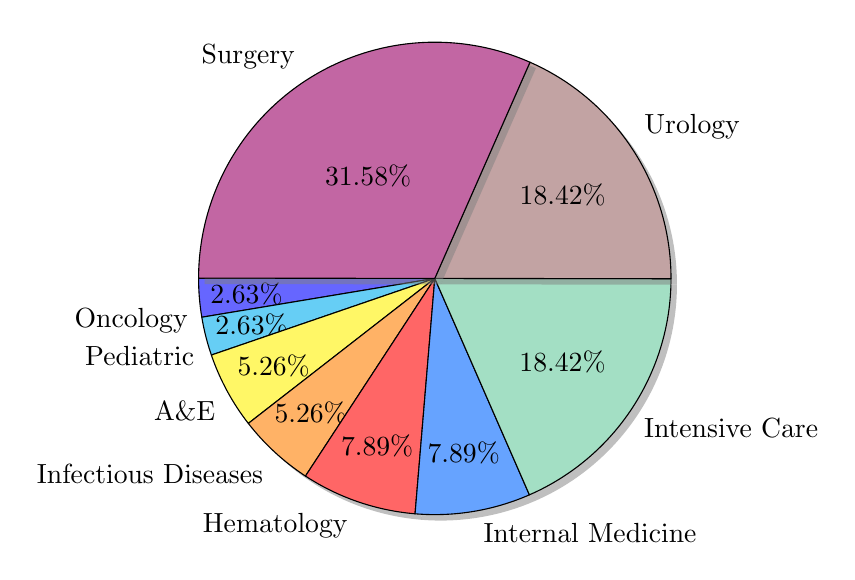
\begin{tikzpicture}
\pie [
	radius = 3,
	rotate = 180,
	style=drop shadow
]{2.63/Oncology, 2.63/Pediatric, 5.26/A\&E, 5.26/Infectious Diseases, 7.89/Hematology, 7.89/Internal Medicine, 18.42/Intensive Care, 18.42/Urology, 31.58/Surgery}
\end{tikzpicture}
\caption{Origin of the samples: Ward}
\label{wards}
\end{figure}

The samples were mainly rectal swabs (\emph{42,11$\%$}), blood samples (\emph{26,32$\%$}), and urine samples (\emph{18,42$\%$}) (Figure \ref{clinical_mat}).

\begin{figure}[h!]
\centering
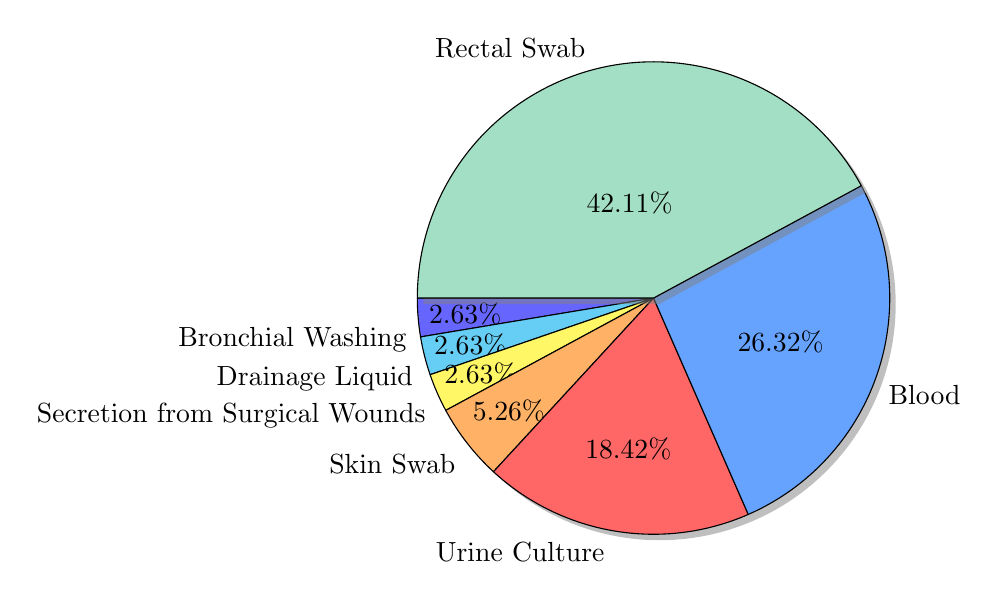
\begin{tikzpicture}
\pie [
radius = 3,
rotate = 180,
style=drop shadow
] {2.63/Bronchial Washing, 2.63/Drainage Liquid, 2.63/Secretion from Surgical Wounds, 5.26/Skin Swab, 18.42/Urine Culture, 26.32/Blood, 42.11/Rectal Swab}
\end{tikzpicture}
\caption{Origin of the samples: Clinical material}
\label{clinical_mat}
\end{figure}

\clearpage

After the on plate isolation of pure colonies, in order to identify the antibiotic resistances, phenotypic tests were performed using the \emph{VITEK}\textsuperscript{\textregistered}\emph{2}.
All the samples analysed were resistant to Piperacillin/Tazobactam and Cefotaxime, while antibiotics that still show a certain degree of effectiveness are Colistin, Fosfomycin, and Amikacin.
Among the thirty-eight samples, the \emph{21$\%$} showed resistances to all the antibiotics tested (Figure \ref{vitek})

\begin{figure}[h!]
\centering
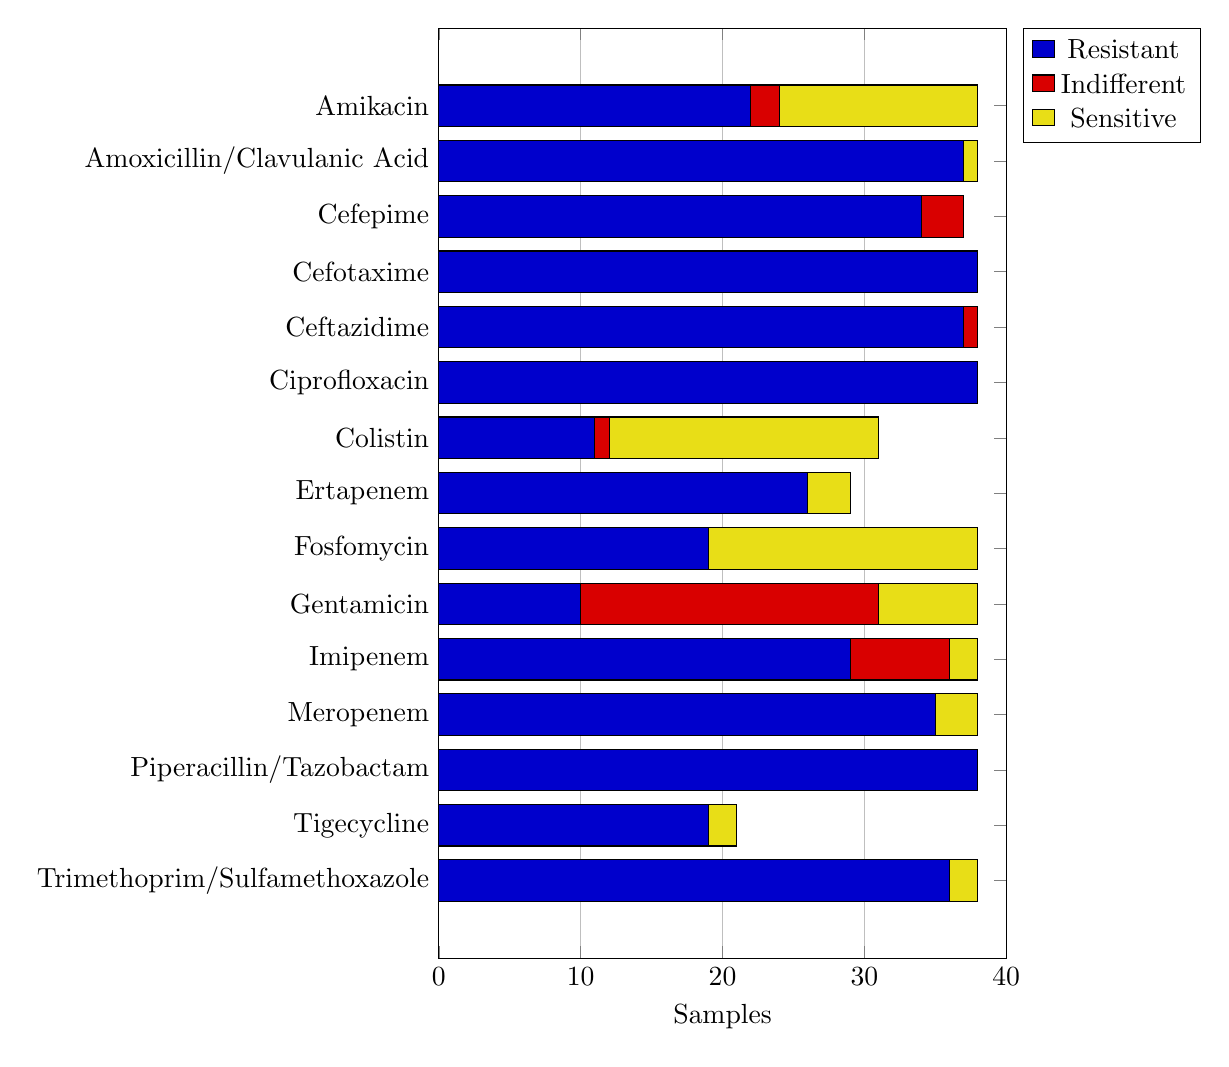
\begin{tikzpicture}
\begin{axis}[
xbar stacked,
xmin=0,
y=20pt,
width=250pt,
bar shift=0pt,
xmajorgrids,
bar width=15pt,
xlabel={Samples},
symbolic y coords={
	Trimethoprim/Sulfamethoxazole,
	Tigecycline,
	Piperacillin/Tazobactam,
	Meropenem,
	Imipenem,
	Gentamicin,
	Fosfomycin,
	Ertapenem,
	Colistin,
	Ciprofloxacin,
	Ceftazidime,
	Cefotaxime,
	Cefepime,
	Amoxicillin/Clavulanic Acid,
	Amikacin
},legend pos=outer north east,
ytick=data,
xmax=40
]

%Blue bars = resistant
\addplot [black, fill=black!20!blue, mark=none] coordinates {
	(22,Amikacin)
	(37,Amoxicillin/Clavulanic Acid)
	(34,Cefepime)
	(38,Cefotaxime)
	(37,Ceftazidime)
	(38,Ciprofloxacin)
	(11,Colistin)
	(26,Ertapenem)
	(19,Fosfomycin)
	(10,Gentamicin)
	(29,Imipenem)
	(35,Meropenem)
	(38,Piperacillin/Tazobactam)
	(19,Tigecycline)
	(36,Trimethoprim/Sulfamethoxazole)
};

%Red bars = indifferent
\addplot [black, fill=black!15!red, mark=none] coordinates {
	(2,Amikacin)
	(0,Amoxicillin/Clavulanic Acid)
	(3,Cefepime)
	(0,Cefotaxime)
	(1,Ceftazidime)
	(0,Ciprofloxacin)
	(1,Colistin)
	(0,Ertapenem)
	(0,Fosfomycin)
	(21,Gentamicin)
	(7,Imipenem)
	(0,Meropenem)
	(0,Piperacillin/Tazobactam)
	(0,Tigecycline)
	(0,Trimethoprim/Sulfamethoxazole)
};


%Yellow bars = sensitive
\addplot [black, fill=black!10!yellow, mark=none] coordinates {
(14,Amikacin)
(1,Amoxicillin/Clavulanic Acid)
(0,Cefepime)
(0,Cefotaxime)
(0,Ceftazidime)
(0,Ciprofloxacin)
(19,Colistin)
(3,Ertapenem)
(19,Fosfomycin)
(7,Gentamicin)
(2,Imipenem)
(3,Meropenem)
(0,Piperacillin/Tazobactam)
(2,Tigecycline)
(2,Trimethoprim/Sulfamethoxazole)
};

\legend{Resistant, Indifferent, Sensitive}
\end{axis}
\end{tikzpicture}
\caption{Determination of antibiotic resistance/sensitivity profile with \emph{VITEK}\textsuperscript{\textregistered}\emph{2}}
\label{vitek}
\end{figure}

\clearpage

After the phenotypic identification, the colonies were subjected to genotypic analysis to identify which antibiotic-resistant molecules were produced by the bacteria.

Among the thirty-eight samples, thirty-four were KPC positive, while two samples were OXA-48 positive.
No sample (\emph{0$\%$}) was found to produce VIM, IMP or NDM carbapenemases (Figure \ref{genexpert}).

\begin{figure}[h!]
\centering

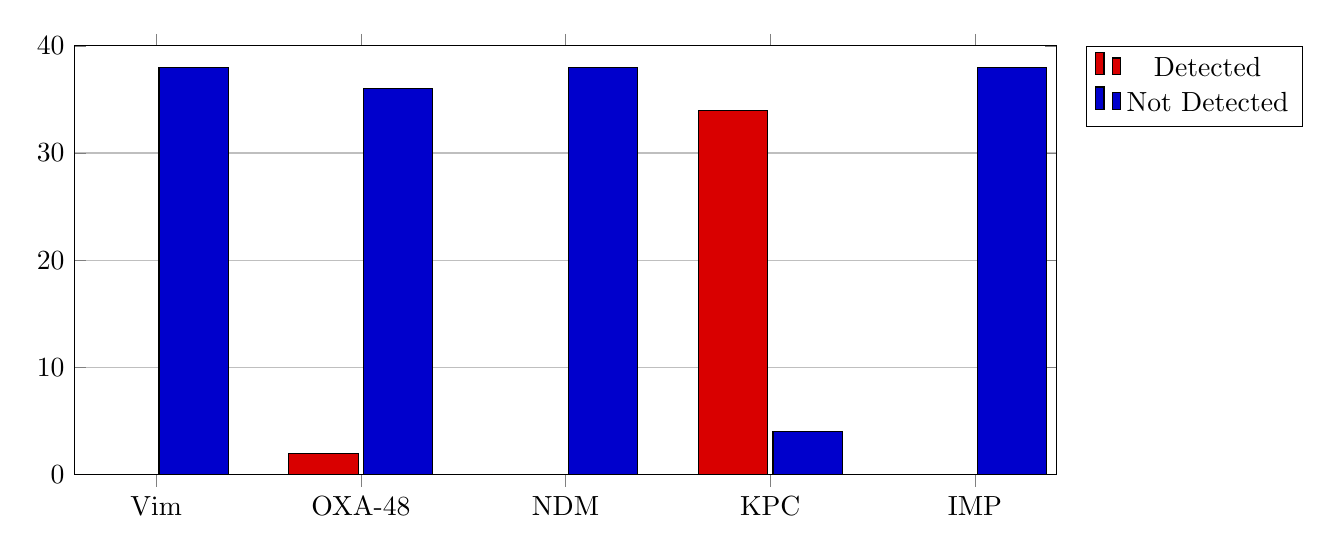
\begin{tikzpicture}
\begin{axis}[
ybar,
ymin=0,
ymajorgrids,
bar width=25pt,
width=400pt,
height=200pt,
symbolic x coords={
	Vim,
	OXA-48,
	NDM,
	KPC,
	IMP
},
legend pos=outer north east,
xtick=data,
ymax=40,
]
\addplot [black, fill=black!15!red, mark=none] coordinates {
	(IMP,0)
	(KPC,34)
	(NDM,0)
	(OXA-48,2)
	(Vim,0)
};

\addplot [black, fill=black!20!blue, mark=none] coordinates {
	(IMP,38)
	(KPC,4)
	(NDM,38)
	(OXA-48,36)
	(Vim,38)
};

\legend{Detected, Not Detected}
\end{axis}
\end{tikzpicture}
\caption{Determination of genotypic variants with \emph{GeneXpert}}
\label{genexpert}
\end{figure}

\chapter{Final considerations}

As the ``Surveillance report'' of 2015 has highlighted, Italy reports a carbapenem resistance percentage of 33$\%$, making it one of the most affected by this issue \cite{ECDC_Surveillance}.

All the samples analysed during this work showed antibiotic resistances, proving to be in line with the national data.

The increasing spread of antimicrobial-resistant \emph{K. pneumoniae} has become a public health concern of growing importance in Europe.

In order to deal with this problem, measures such as timely and appropriate laboratory reporting, screening and isolation of high-risk patients, and better infection control should be implemented.

The data collected during this work showed that, among the carbapenemases producing strains analysed, the most represented were KPC carbapenemases.

Since the growing spread of these antibiotic resistances is influenced by the selective pressure of broad-spectrum antibiotic therapies, this work has taken into account also the antibiotic-resistances profiles, questioning the efficacy of current therapies.
 
Even if the small number of samples analysed can't be considered statistically significant, the data collected shows that the efficacy of the most common antibiotics currently used is seriously compromised.

Given that \emph{Enterobacteriaceae} infections are associated with higher health-care costs, prolonged hospital stays, treatment failure and mortality, the role of microbiology laboratories is fundamental to monitor the spread of such bacteria in hospital settings, and its resulting clinical implications.

\bibliography{references}
\bibliographystyle{unsrt}

\end{document}http://www.lorenzopantieri.net/LaTeX_files/ArteLaTeX.pdf